\section{Introduction}
\label{sec:intro}

The field of video generation has transitioned from synthesizing blurry, single-shot clips to attempting complex, cinematic multi-shot narratives (Text-to-Multi-Shot Video, T2MSV). However, evaluation methodologies remain anchored in a single-shot mindset. Existing metrics, such as Fréchet Video Distance (FVD) or frame-wise CLIP similarity, evaluate videos holistically. In multi-shot environments, this holistic approach introduces a critical vulnerability: it inadvertently rewards models that generate entirely static, unchanging videos, even when explicitly prompted to execute dynamic scene transitions.

\begin{figure}[ht]
    \centering
    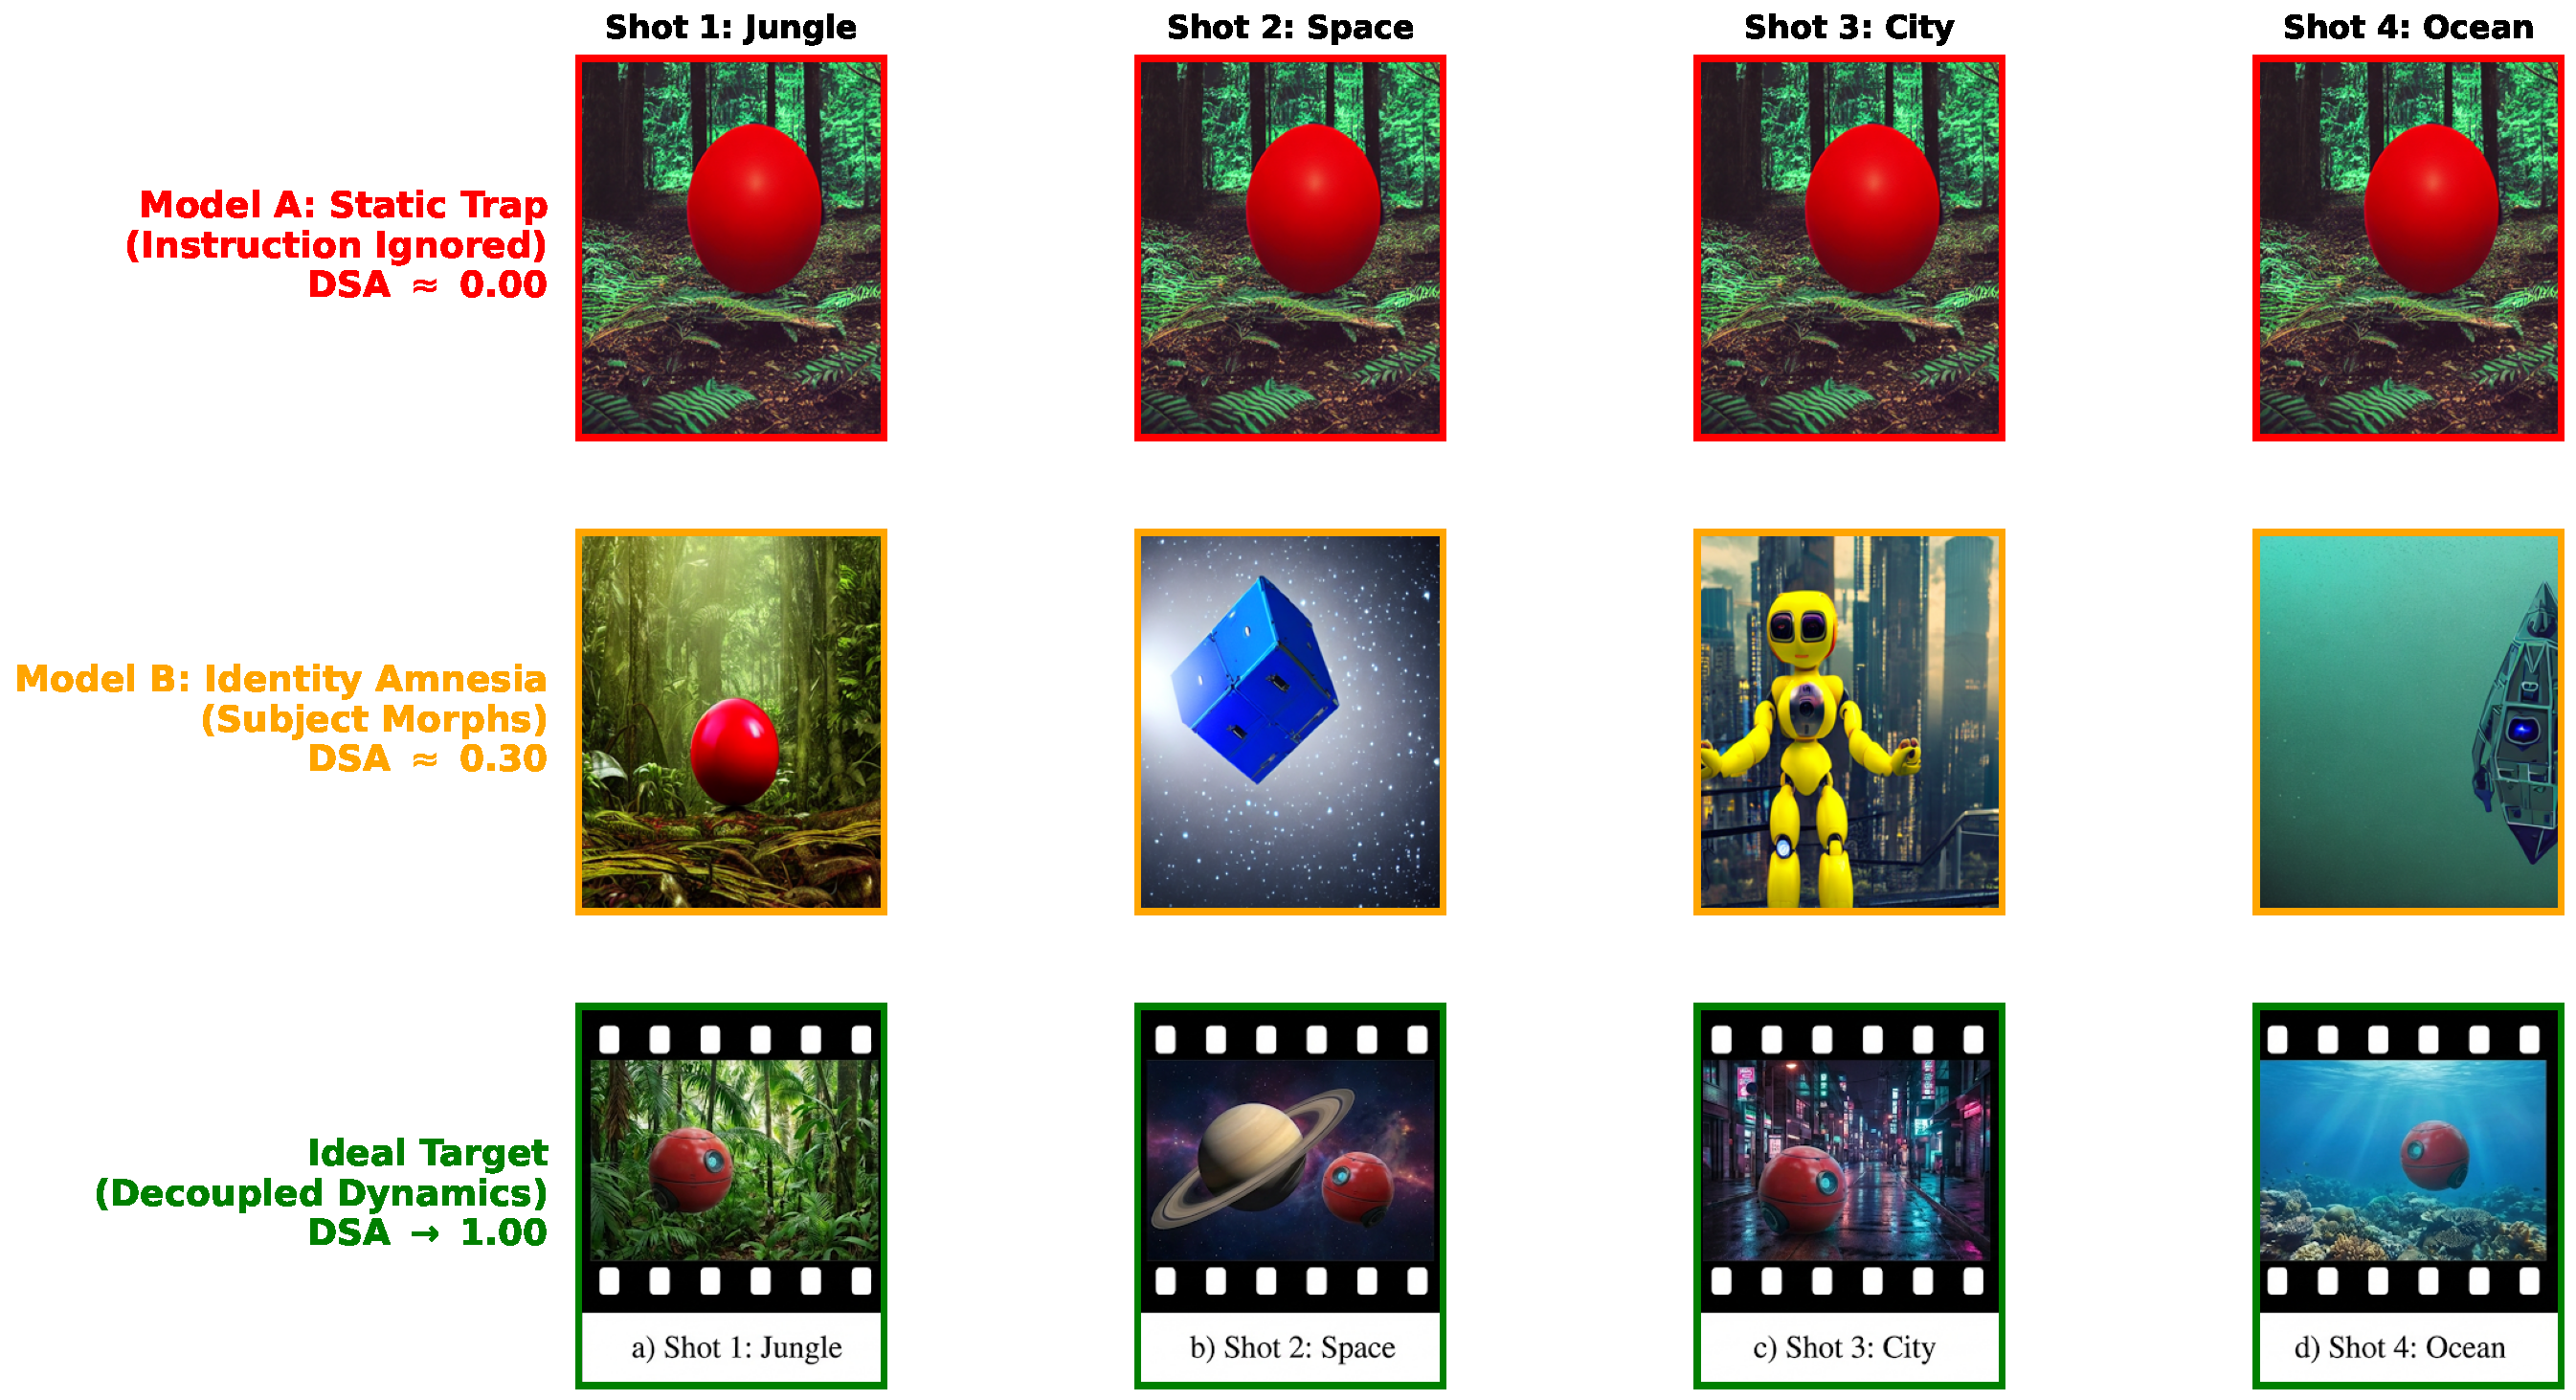
\includegraphics[width=\linewidth]{figures/fig1_teaser_robot.pdf}
    \caption{The dilemma of current T2MSV models illustrated with a "Retro-futuristic Robot" scenario. (A) \textbf{Static Trap}: The model (e.g., CogVideoX) maintains high consistency by ignoring background change instructions, repeating the jungle environment across all shots. (B) \textbf{Identity Amnesia}: The model (e.g., StoryDiffusion) executes transitions but fails to preserve the robot's specific geometry and color. (C) \textbf{Ideal Goal}: Our proposed benchmark demands both radical dynamics and strict identity preservation.}
    \label{fig:teaser}
\end{figure}

We define this phenomenon as the \textbf{Static Video Trap}. When a prompt demands a sequence jumping from a "rainforest" to "outer space," a model that stubbornly remains in the rainforest will score artificially high on traditional temporal consistency metrics. This creates the \textbf{Global Similarity Paradox}: metrics inherently reward the failure to transition. Conversely, models attempting to dynamically execute the transition often suffer from \textbf{Identity Amnesia}, losing the fine-grained visual features of the main subject.

In this work, we argue that T2MSV requires the precise management of \textit{intended discontinuities}. We introduce \textbf{Dynamic-MSV-Bench}, a comprehensive evaluation framework that disentangles subject identity from environmental dynamics across two critical tracks:
\begin{itemize}
    \item \textbf{Track S (Semantic Leap):} Tests narrative diversity, requiring radical environment changes while strictly preserving the subject.
    \item \textbf{Track M (Motion Continuity):} Evaluates spatial integrity, where the background must remain perfectly consistent while the camera executes specific motions.
\end{itemize}

Our core contributions are:
\begin{itemize}
    \item We expose the \textbf{Static Trap} and \textbf{Amnesia Trap}, highlighting the fundamental flaws of legacy temporal metrics that penalize intended cinematic cuts and semantic shifts.
    \item We propose a 4D decoupled evaluation pipeline (assessing subject identity, background dynamics, cut sharpness, and instruction alignment), introducing \textbf{Diagonal Semantic Alignment (DSA)}, which assigns a strict zero score to static, instruction-ignoring videos.
    \item We empirically demonstrate that neither Foundation T2V models nor specialized T2MSV inference frameworks have solved the underlying "Double-Kill" dilemma of multi-shot generation.
\end{itemize}